\documentclass[class=report,crop=false, 12pt]{standalone}
\usepackage[screen,nosolutions]{../scratch}

%\usepackage[print]{../scratch}

\begin{document}

\titre[S]{Si ... alors ...}
%===============================

\insertvideo{pHK3fOJ52Ls}{Si ... alors ... -- Activité 1}

\insertvideo{zXS6NXVUeiQ}{Si ... alors ... -- Activité 2}

\insertvideo{m0YvDz-f3SE}{S i... alors ... -- Activité 3}

\bigskip
\bigskip

\begin{activite}

Scratch se déplace et rebondit sur les bords, il doit atteindre le disque rouge sans toucher les rectangles bleus. Pour cela, il faut choisir la bonne orientation initiale.

\begin{center}
  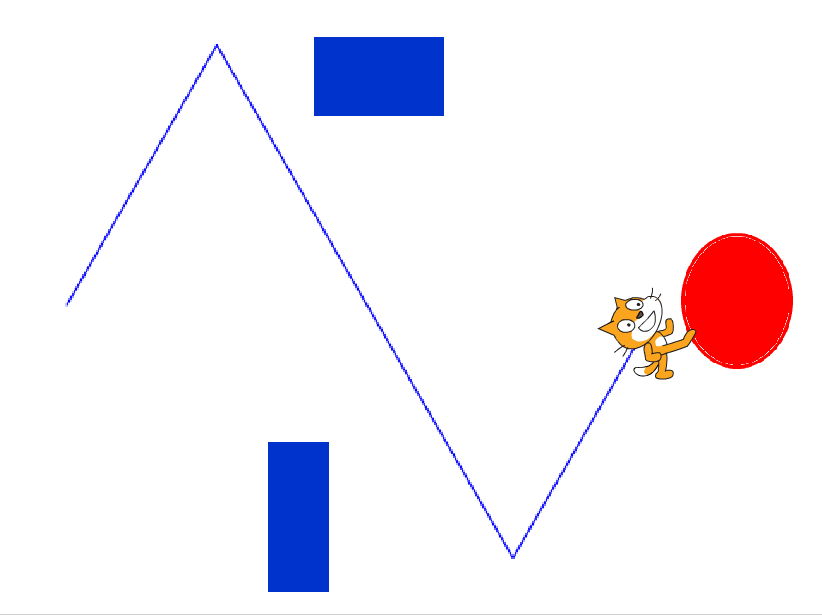
\includegraphics[scale=\scaleecran]{ecran-04-ex1} 
\end{center}

\begin{enumerate}
  \item Scratch part de $x=-200$, $y=0$. Il s'oriente selon un certain angle (par exemple $30$\textdegree). Puis dans une boucle \og répéter indéfiniment \fg{} : il avance un peu (disons $5$ pas) et il \og rebondit si le bord est atteint \fg{}.
  
  
  \item Complète la boucle précédente pour tester si Scratch touche une zone colorée :
  \begin{itemize}
    \item si Scratch touche une zone rouge alors c'est gagné et on arrête le programme,
    
    \item si Scratch touche une zone bleue alors c'est perdu et on arrête aussi le programme.
  \end{itemize}
   
  \item Dessine des obstacles (en bleu) et une cible (en rouge) sur l'arrière-plan. Cherche l'angle de départ qui convient à la fois pour éviter les obstacles et pour atteindre la cible !
\end{enumerate}



\textbf{Blocs utiles.}
\begin{center}
  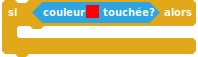
\includegraphics[scale=\scalebloc]{bloc-04-ex1a}  \qquad
  
\includegraphics[scale=\scalebloc]{bloc-04-ex1b}   
\end{center}


\end{activite}


\begin{activite}

L'utilisateur déplace Scratch avec les touches de flèches du clavier, de façon à suivre un chemin.

\begin{center}
  
\includegraphics[scale=\scaleecran,scale=1.4]{ecran-04-ex2} 
\end{center}

\begin{enumerate}
  \item Dans une boucle sans fin, on teste quelle flèche est pressée.
  Si c'est la flèche du haut, Scratch monte (de 5 pas par exemple). Si c'est la flèche du bas, Scratch descend...
  
  \item Dessine un parcours sur l'arrière-plan : tout d'abord peins tout le fond en bleu (avec l'outil pot de peinture) ; puis avec l'outil pinceau (en grande taille) trace un chemin d'une autre couleur.
  
  \item Réduis la taille du lutin Scratch afin qu'il puisse parcourir le chemin sans toucher les bords colorés.
  
  \item \textbf{Bonus.} Si Scratch sort de son chemin, joue un son d'alerte.
\end{enumerate}


\textbf{Blocs utiles.}
\begin{center}
  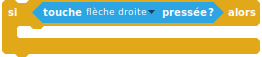
\includegraphics[scale=\scalebloc]{bloc-04-ex2} 
\end{center}


\end{activite}


\begin{activite}

Il s'agit de programmer un jeu : 
\begin{itemize}
  \item Scratch part de la gauche de l'écran, il est visible.
  \item Au bout de quelques pas, il disparaît mais continue d'avancer. 
  \item Lorsque le joueur appuie sur le bouton gauche de la souris, Scratch s'arrête et réapparaît.
  \item Si Scratch touche la barre noire à ce moment là, c'est gagné !
\end{itemize}

\begin{center}
  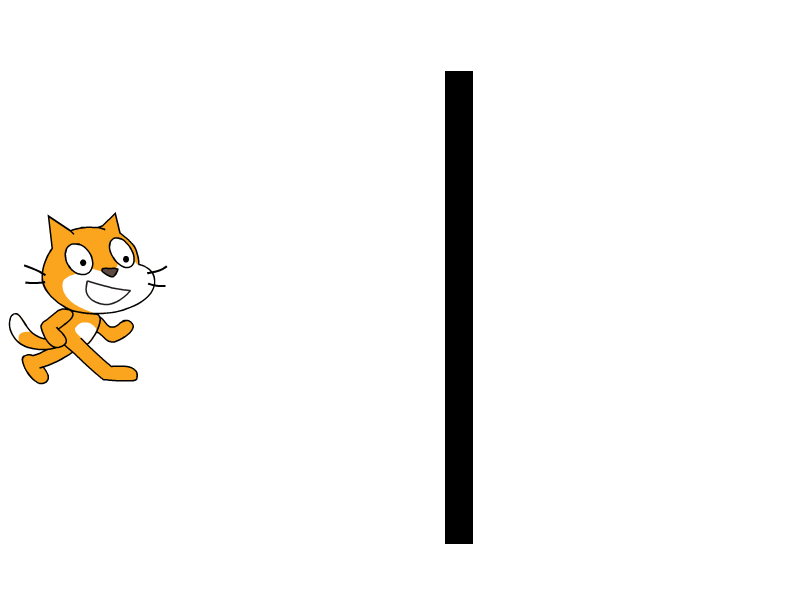
\includegraphics[scale=\scaleecran]{ecran-04-ex3} 
\end{center}

Dans un premier temps, modifie l'arrière-plan pour y dessiner une barre verticale noire vers le milieu de l'écran.

\begin{enumerate}
  \item \textbf{Première partie.} Scratch démarre.
  
  \begin{itemize}
    \item Positionne Scratch à gauche de l'écran, visible.
    \item Répète 10 fois : Scratch avance de 5 et attend un peu (par exemple 0,1 seconde). 
  \end{itemize}
  
  
  \item \textbf{Deuxième partie.} Scratch se cache.
  
  \begin{itemize}
    \item Cache Scratch.
    \item Répète 70 fois : Scratch avance de 5 et attend un peu (le même temps qu'avant). 
  \end{itemize}
  
  \item \textbf{Troisième partie.} Le joueur clique.
  
  Dans chaque itération de la boucle précédente, on teste si le bouton gauche de la souris est pressé. Si le joueur clique sur la souris alors :
  \begin{itemize}
    \item Montre Scratch.  
    \item Si Scratch touche la barre noire alors affiche : \og c'est gagné ! \fg{}.
    \item Arrête le programme.
  \end{itemize}  
\end{enumerate}

\bigskip
\textbf{Blocs utiles.}
\begin{center}
  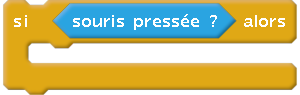
\includegraphics[scale=\scalebloc]{bloc-04-ex3a}\quad
  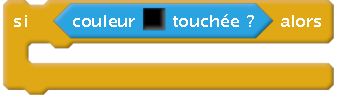
\includegraphics[scale=\scalebloc]{bloc-04-ex3b}\quad
  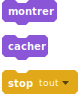
\includegraphics[scale=\scalebloc]{bloc-04-ex3c}    
\end{center}

\end{activite}



\ifx \displaysolutions \myzero
\else
\begin{code}
\onesolution{Si ... alors ...}{Activité 1}{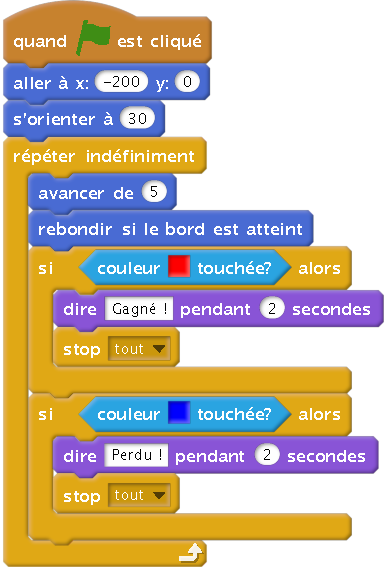
\includegraphics[scale=\scalesolution]{code-04-ex1}}
\onesolution{Si ... alors ...}{Activité 2}{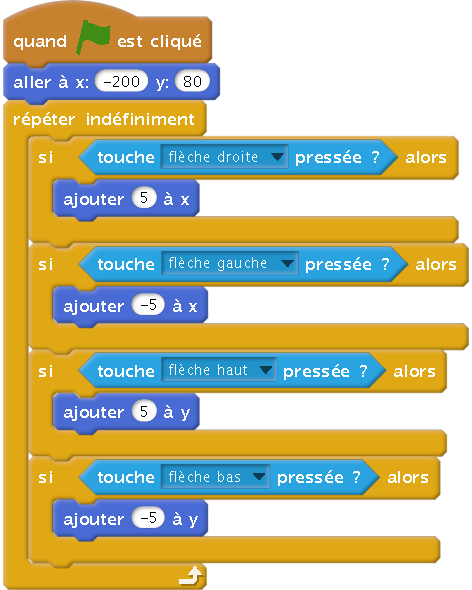
\includegraphics[scale=\scalesolution]{code-04-ex2}}
\onesolution{Si ... alors ...}{Activité 3}{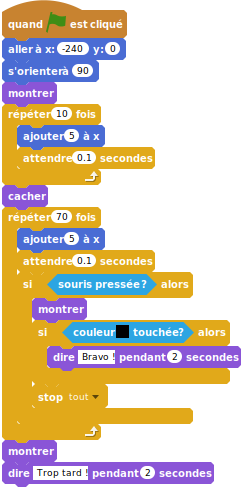
\includegraphics[scale=\scalesolution]{code-04-ex3}}    
\end{code}
\fi



\end{document}

